\documentclass{article}%
\usepackage[T1]{fontenc}%
\usepackage[utf8]{inputenc}%
\usepackage{lmodern}%
\usepackage{textcomp}%
\usepackage{lastpage}%
\usepackage[head=40pt,margin=0.5in,bottom=0.6in]{geometry}%
\usepackage{graphicx}%
%
\title{\textbf{Denuncian que calles de Candelaria amanecieron con montañas de basura}}%
\author{MIGDALIS CAÑIZALEZ V.}%
\date{16/09/2018}%
%
\begin{document}%
\normalsize%
\maketitle%
\textbf{URL: }%
http://www.eluniversal.com/caracas/20786/denuncian{-}que{-}calles{-}de{-}candelaria{-}amanecieron{-}con{-}montanas{-}de{-}basura\newline%
%
\textbf{Periodico: }%
EU, %
ID: %
20786, %
Seccion: %
caracas\newline%
%
\textbf{Palabras Claves: }%
NO\_TIENE\newline%
%
\textbf{Derecho: }%
3.2, %
Otros Derechos: %
, %
Sub Derechos: %
3.2.1\newline%
%
\textbf{EP: }%
NO\newline%
\newline%
%
\textbf{\textit{Los vecinos de esta parroquia informaron que los camiones de recolección no han  pasado  por la zona, por lo que en cada esquina hay desechos}}%
\newline%
\newline%
%
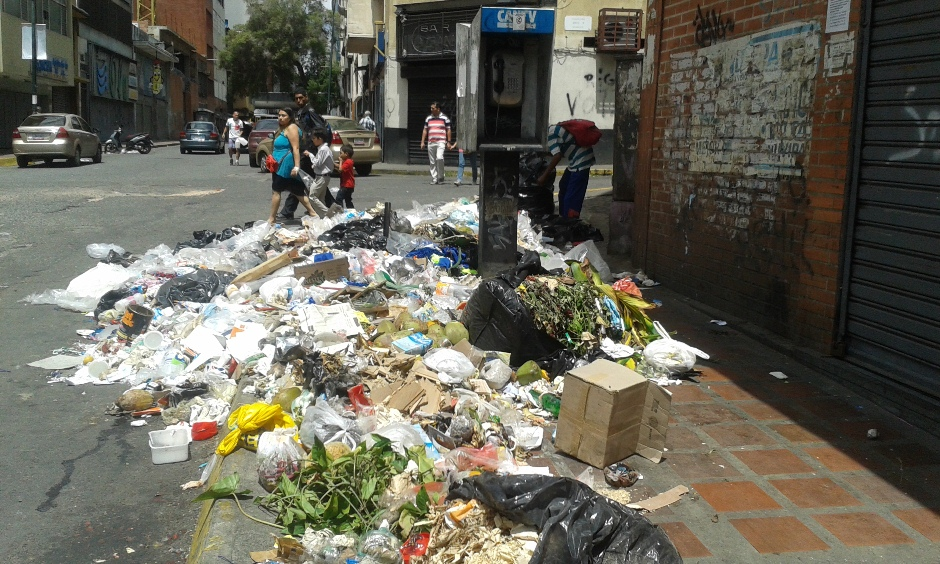
\includegraphics[width=300px]{23.jpg}%
\newline%
%
Este domingo en cada esquina de Candelaria se encuentran montañas de basura debido a que los camiones no han pasado desde el pasado viernes, según Mariana Rojas, vecina del sector.%
\newline%
%
En la esquina de Ferrenquin, frente a la sede del Ministerio Público, los desechos están en medio de las aceras. También en la esquina de Manduca la situación es similar.%
\newline%
%
Según denuncia, el servicio de aseo en el sector es muy irregular y eso se une a la cantidad de indigentes que circulan por la zona y que rompen las bolsas para hurgar la basura.%
\newline%
%
\end{document}